\begin{center}
    \Large{\textbf{Відповіді на контрольні питання}}    
\end{center}

\vspace{1mm}

\begin{enumerate}
    \item Що таке інтерференція світлових хвиль?
    \bigbreak
    Інтерференція - явище накладання когерентних світлових хвиль при якому спостерігається перерозподіл світлового потоку в просторі.

    \item Як отримати інтерференцію світла за допомогою плоскопаралельної пластини?
    \bigbreak

    Інтерференцію світла за допомогою плоскопаралельної пластини
    можна отримати за допомогою методу ділення амплітуди, коли
    пучок поділяється на дві або декілька частин  за 
    допомогою відбиваючих, частинно прозорих поверхонь.

    \begin{figure}[h]
        \centering
        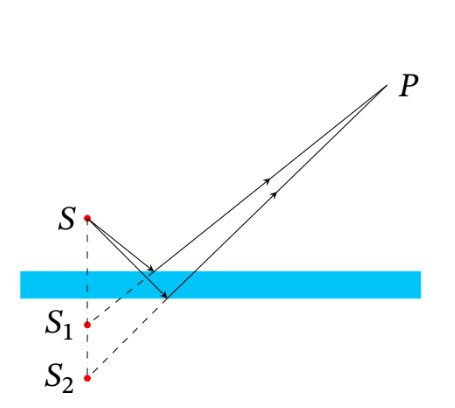
\includegraphics[width=0.3\textwidth]{assets/separate_amplitude.png}
    \end{figure}

    \item Яким чином утворюються уявні джерела світла? Навіщо стоїть 
    короткофокусна лінза на виході джерела світла у схемі нашої роботи?
    \bigbreak

    Уявні джерела можливо утворювати за допомогою лінз,
    які будуть розподіляти світло таким чином, як би це було,
    якщо десь існувало інше джерело(уявн). Наприклад,
    у нашій роботі(рис. 1) світловий промінь від лазера
    проходить через короткофокусну лінзу, змонтовану в центрі
    екрана. Тому процес розсіяння світла можна розглядати
    як утворення уявного точкового джерела когерентного
    випромінювання.

    \item Що таке когeрентність хвиль? Просторова і часова когерентність.
    \bigbreak
    Когерентність - це здатність хвиль до інтерференції(вони мають 
    однакову частоту і в точках накладання - сталу різницю фаз)

    Просторова когерентність - когерентність коливань,
    які відбуваються у один і той же момент часу
    у різних точках площини, пенпендикул в разных точках плоскости, перпендикулярной направлению распространения волны.яній напрямку поширення хвилі.
    
    Часова когерентність - когерентність коливань, які відбуваються у одній області, але
    відстають один від одного на певний обмежений обмежений проміжок часу.
    
    \item Інтерференція на тонких плівках. Чому ми бачимо різні кольори світла?
    \bigbreak
    
    Інтерференція на тонких плівках - виникнення стійкої інтерференційної 
    картини при відбиванні променів від поверхонь шару прозорої речовини,
    товщина якого не перебільшує 40 мкм.
    Оскільки явище інтерференції напряму залежить від довжини хвилі, то
    при інтерференції світла, що містить різні спектральні складові, наприклад,
    білого світла, відбувається розділення цих спектральних складових, і ми
    бачимо веселкові смуги.

    
    \item Апертура інтерференції і пучків.
    \bigbreak

    Апертура інтерференції - кут, під яким виходять
    з джерела світла промені, що інтерферують  на екрані.
    Вона визначає, чи буде можливість спостерігати 
    явище інтерференції. Максимальне значення, за якого ще
    будемо спостерігати інтерференцію дорівнює відношенню
    довжини хвилі до розміру джерела світла. 

    Апертура пучка - (в геометричній оптиці) визначає розмір
    цього пучка променів.

    \item Що таке інтерференція світла зі смугами рівної товщини, рівного нахилу?
    \bigbreak

    Інтерференційні смуги або кільця, що виникають
    через різниці ходу між окремими парами вторинних променів, з
    яких кожна пара походить від різних точок джерела світла називаються смугами рівного нахилу.
    Смуги рівного нахилу спостерігаються в тих випадках,
    коли на тонку плоскопаралельну пластинку падає під різними
    кутами пучок світла, що розбігається чи збігається. 
    Умови інтерференції є однакові для всіх променів, що 
    падають на поверхню пластинки й відбиваються від неї під 
    одним і тим самим кутом.
 
    Інтерференційними смугами рівної товщини називаються інтерференційні смуги, які утворюються в результаті зміни променів в області
    перетину вторинних променів,
    що виникають з одного первинного променя.
    Смуги рівної товщини спостерігаються при відбиванні 
    паралельного пучка світлових променів від тонкої прозорої
    пластинки, товщина якої неоднакова в різних місцях. Умови максимуму 
    інтерференції є однакові в точках, що відповідають 
    однаковим значенням товщини.
    



\end{enumerate}